\chapter{InfoNCE and Contrastive Predictive Coding}
\label{chap:infonce}

\section{Introduction and Intuition}

One of the most persistent challenges in unsupervised and self-supervised representation learning is the problem of modeling high-dimensional, complex data such as raw audio waveforms, natural images, or streams of text. Traditional generative models typically attempt to reconstruct the input data directly, pixel by pixel or sample by sample, relying on maximum likelihood estimation over the entire observation space. While mathematically appealing, this approach fundamentally forces the model to allocate significant capacity to modeling low-level noise and microscopic details that are often irrelevant to the underlying semantic content. The true signal---the macroscopic structure and meaning---is easily drowned out.

Contrastive Predictive Coding (CPC), introduced by Oord et al., offers an elegant, information-theoretic alternative: rather than predicting the exact future observations in the original high-dimensional space, the model extracts a compact latent representation and performs predictions strictly within that lower-dimensional space. By doing so, the model is encouraged to discard local noise and retain only the "slow features" that evolve over time and hold semantic meaning.

To prevent the model from arriving at the trivial solution (i.e., the encoder mapping all inputs to a constant vector), CPC employs a contrastive learning objective. The model is tasked with distinguishing the true future observation (the "positive" sample) from a set of randomly drawn observations (the "negative" samples). This discrimination task requires the latent representations to capture the shared information between the present context and the future observation. 

The loss function that formalizes this objective is known as Information Noise-Contrastive Estimation (InfoNCE). Remarkably, as we will demonstrate rigorously in this chapter, minimizing the InfoNCE loss is mathematically equivalent to maximizing a lower bound on the mutual information between the context and the future observations. This connects a practical, empirically successful representation learning technique directly to the foundational principles of information theory discussed in Part I.

\section{Formalizing Contrastive Predictive Coding}

Let us formalize the setting. Consider a sequence of observations $\mathbf{x} = (x_1, x_2, \dots, x_T)$ where each $x_t \in \mathcal{X}$. In practice, $\mathcal{X}$ might be a patch of an image, a window of a speech waveform, or a token in a sentence.

\begin{definition}[CPC Architecture]
A Contrastive Predictive Coding architecture consists of two parametric mappings:
\begin{enumerate}
    \item An \textbf{encoder} (or inference model) $z_t = f_\theta(x_t)$, where $f_\theta : \mathcal{X} \to \mathbb{R}^d$, mapping high-dimensional observations into a latent representation sequence.
    \item An \textbf{autoregressive model} $c_t = g_\phi(z_{\le t})$, where $g_\phi : (\mathbb{R}^d)^* \to \mathbb{R}^c$, summarizing the present and past latent variables into a context vector $c_t$.
\end{enumerate}
\end{definition}

The objective is to predict future latent states $z_{t+k}$ for some horizon $k>0$, given the current context $c_t$. Instead of training a full generative model $p_\theta(z_{t+k} | c_t)$, CPC models a density ratio which preserves the mutual information $I(x_{t+k}; c_t)$.

\begin{figure}[htbp]
\centering
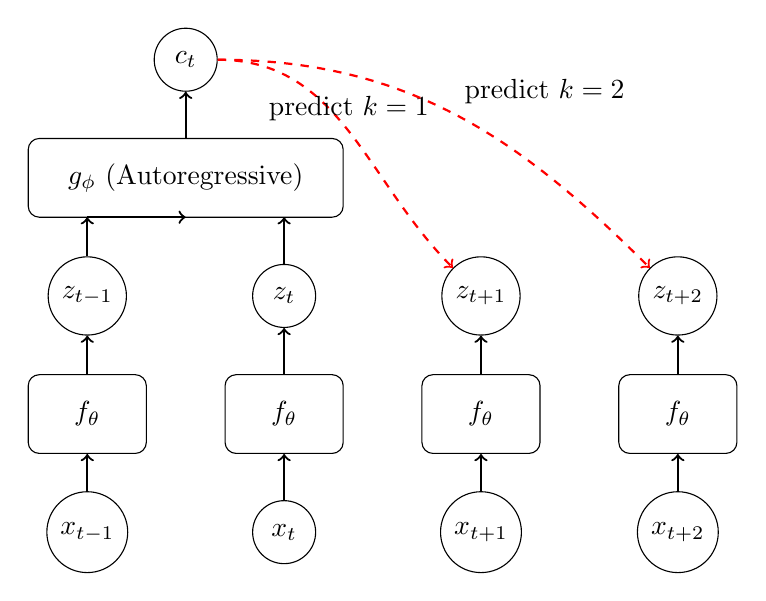
\begin{tikzpicture}[
    block/.style={rectangle, draw, rounded corners, text centered, minimum width=1.5cm, minimum height=1cm},
    circ/.style={circle, draw, text centered, minimum size=0.8cm},
    arrow/.style={->, thick}
]

% Inputs
\node[circ] (x1) at (0, 0) {$x_{t-1}$};
\node[circ] (x2) at (2.5, 0) {$x_t$};
\node[circ] (x3) at (5, 0) {$x_{t+1}$};
\node[circ] (x4) at (7.5, 0) {$x_{t+2}$};

% Encoder
\node[block] (enc1) at (0, 1.5) {$f_\theta$};
\node[block] (enc2) at (2.5, 1.5) {$f_\theta$};
\node[block] (enc3) at (5, 1.5) {$f_\theta$};
\node[block] (enc4) at (7.5, 1.5) {$f_\theta$};

% Latents
\node[circ] (z1) at (0, 3) {$z_{t-1}$};
\node[circ] (z2) at (2.5, 3) {$z_t$};
\node[circ] (z3) at (5, 3) {$z_{t+1}$};
\node[circ] (z4) at (7.5, 3) {$z_{t+2}$};

% AR model
\node[block, minimum width=4cm, minimum height=1cm] (ar) at (1.25, 4.5) {$g_\phi$ (Autoregressive)};
\node[circ] (ct) at (1.25, 6) {$c_t$};

% Arrows
\draw[arrow] (x1) -- (enc1); \draw[arrow] (enc1) -- (z1);
\draw[arrow] (x2) -- (enc2); \draw[arrow] (enc2) -- (z2);
\draw[arrow] (x3) -- (enc3); \draw[arrow] (enc3) -- (z3);
\draw[arrow] (x4) -- (enc4); \draw[arrow] (enc4) -- (z4);

\draw[arrow] (z1) -- (0, 4);
\draw[arrow] (z2) -- (2.5, 4);
\draw[arrow] (0,4) -- (0, 4.0) -- (1.25, 4.0);

\draw[arrow] (ar.north) -- (ct);

\draw[arrow, dashed, red] (ct.east) to[out=0, in=135] node[midway, above, text=black] {predict $k=1$} (z3.north west);
\draw[arrow, dashed, red] (ct.east) to[out=0, in=135] node[midway, above right, text=black] {predict $k=2$} (z4.north west);

\end{tikzpicture}
\caption{The Contrastive Predictive Coding architecture. High-dimensional inputs $x$ are mapped to latents $z$. An autoregressive model aggregates past latents into a context $c_t$, which is used to predict future latents via a contrastive loss.}
\label{fig:cpc_arch}
\end{figure}

\section{The InfoNCE Loss and Mutual Information Bound}

To train the encoder $f_\theta$ and the autoregressive model $g_\phi$, we optimize the InfoNCE loss. Let us define a scoring function $f(x, c)$ which measures the compatibility between a future observation $x$ and a context $c$. Commonly, a log-bilinear form is used: $f(x, c) = \exp(z^T W c)$, where $z = f_\theta(x)$ and $W$ is a learnable weight matrix for the specific step $k$.

\begin{definition}[InfoNCE Loss]
\label{def:infonce}
Given a context $c$ and a set of $N$ samples $X = \{x_1, x_2, \dots, x_N\}$. Assume exactly one sample $x^+ \in X$ is the true future observation drawn from the conditional distribution $p(x | c)$, and the remaining $N-1$ samples are "negative" samples drawn from a proposal distribution, typically the marginal $p(x)$. The InfoNCE loss is defined as:
\begin{equation}
    \mathcal{L}_{\text{InfoNCE}} = - \mathbb{E}_{X} \left[ \log \frac{f(x^+, c)}{\sum_{x_j \in X} f(x_j, c)} \right]
\end{equation}
\end{definition}

Minimizing this loss corresponds to maximizing the probability that the model correctly identifies the true positive sample $x^+$ from the set of candidates $X$.

\begin{figure}[htbp]
\centering
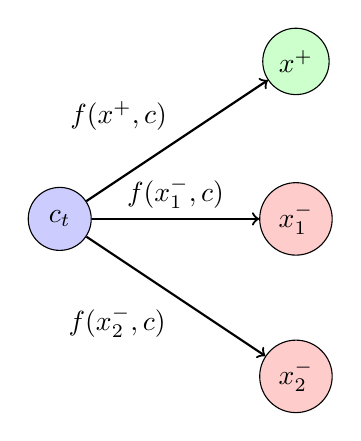
\begin{tikzpicture}[
    circ/.style={circle, draw, text centered, minimum size=0.8cm},
    arrow/.style={->, thick}
]

\node[circ, fill=green!20] (pos) at (0, 2) {$x^+$};
\node[circ, fill=red!20] (neg1) at (0, 0) {$x^-_1$};
\node[circ, fill=red!20] (neg2) at (0, -2) {$x^-_2$};

\node[circ, fill=blue!20] (c) at (-3, 0) {$c_t$};

\draw[arrow] (c) -- (pos) node[midway, above left] {$f(x^+, c)$};
\draw[arrow] (c) -- (neg1) node[midway, above] {$f(x^-_1, c)$};
\draw[arrow] (c) -- (neg2) node[midway, below left] {$f(x^-_2, c)$};

\end{tikzpicture}
\caption{The InfoNCE discrimination task. The context $c_t$ is scored against the true future observation $x^+$ and multiple negative samples $x^-_i$. The objective is to maximize the relative score of the positive sample.}
\label{fig:infonce_task}
\end{figure}

\subsection{Optimal Critic and Density Ratio}

Before we relate the InfoNCE loss to mutual information, we must determine the optimal scoring function $f^*(x, c)$.

\begin{lemma}[Optimal Critic for InfoNCE]
\label{lem:optimal_critic}
Assuming infinite capacity for the scoring function $f(x, c)$, the optimal function that minimizes the InfoNCE loss is proportional to the density ratio:
\begin{equation}
    f^*(x, c) \propto \frac{p(x | c)}{p(x)}
\end{equation}
\end{lemma}

\begin{proof}
Let us consider the InfoNCE loss for a fixed context $c$. The expectation over $X$ can be decomposed into an expectation over the positive sample $x^+$ drawn from $p(x|c)$ and the $N-1$ negative samples drawn independently from $p(x)$. Let $x_1 = x^+$ without loss of generality.
\begin{equation}
    \mathcal{L}_{\text{InfoNCE}}(c) = - \int p(x_1 | c) \prod_{j=2}^N p(x_j) \log \left( \frac{f(x_1, c)}{\sum_{i=1}^N f(x_i, c)} \right) dX
\end{equation}
Because the sum $\sum_{i=1}^N f(x_i, c)$ is symmetric with respect to permutations of the indices, we can rewrite this by summing over all possible assignments of the positive sample to index $k \in \{1, \dots, N\}$:
\begin{equation}
    \mathcal{L}_{\text{InfoNCE}}(c) = - \frac{1}{N} \sum_{k=1}^N \int p(x_k | c) \prod_{j \neq k} p(x_j) \log \left( \frac{f(x_k, c)}{\sum_{i=1}^N f(x_i, c)} \right) dX
\end{equation}
We recognize this as a cross-entropy loss for a classification problem where the posterior probability of the true label being $k$ is given by Bayes' rule:
\begin{equation}
    P(y=k | X, c) = \frac{p(x_k | c) \prod_{j \neq k} p(x_j)}{\sum_{i=1}^N p(x_i | c) \prod_{j \neq i} p(x_j)} = \frac{ \frac{p(x_k|c)}{p(x_k)} }{ \sum_{i=1}^N \frac{p(x_i|c)}{p(x_i)} }
\end{equation}
The cross-entropy loss is minimized when the softmax outputs of our model match the true posterior class probabilities. Thus, we must have:
\begin{equation}
    \frac{f(x_k, c)}{\sum_{i=1}^N f(x_i, c)} = \frac{ \frac{p(x_k|c)}{p(x_k)} }{ \sum_{i=1}^N \frac{p(x_i|c)}{p(x_i)} }
\end{equation}
This implies that $f^*(x, c) \propto \frac{p(x|c)}{p(x)}$.
\end{proof}

\subsection{Mutual Information Bound}

We now present the central theorem of this chapter: the relationship between the InfoNCE loss and mutual information.

\begin{theorem}[InfoNCE Mutual Information Bound]
\label{thm:infonce_bound}
Minimizing the InfoNCE loss maximizes a strict lower bound on the mutual information $I(X; C)$ between the observations and the context. Specifically:
\begin{equation}
    I(X; C) \ge \log(N) - \mathcal{L}_{\text{InfoNCE}}
\end{equation}
\end{theorem}

\begin{proof}
Assume we have the optimal critic $f^*(x, c) = \frac{p(x|c)}{p(x)}$. We substitute this into the definition of the InfoNCE loss (Definition \ref{def:infonce}):
\begin{align*}
    \mathcal{L}_{\text{InfoNCE}}^{\text{opt}} &= - \mathbb{E}_{X} \left[ \log \frac{ \frac{p(x^+|c)}{p(x^+)} }{ \frac{p(x^+|c)}{p(x^+)} + \sum_{j=2}^N \frac{p(x_j|c)}{p(x_j)} } \right] \\
    &= \mathbb{E}_{X} \left[ \log \left( 1 + \frac{p(x^+)}{p(x^+|c)} \sum_{j=2}^N \frac{p(x_j|c)}{p(x_j)} \right) \right]
\end{align*}
Let us rewrite this rigorously without Jensen's approximation first:
\begin{align*}
    \mathcal{L}_{\text{InfoNCE}}^{\text{opt}} &= - \mathbb{E}_{X, c} \left[ \log \frac{ p(x^+|c)/p(x^+) }{ \sum_{i=1}^N p(x_i|c)/p(x_i) } \right] \\
    &= - \mathbb{E}_{X, c} \left[ \log \left( \frac{p(x^+|c)}{p(x^+)} \right) \right] + \mathbb{E}_{X, c} \left[ \log \left( \sum_{i=1}^N \frac{p(x_i|c)}{p(x_i)} \right) \right]
\end{align*}
The first term evaluates to exactly the negative mutual information:
\begin{equation}
    - \mathbb{E}_{x^+, c} \left[ \log \left( \frac{p(x^+|c)}{p(x^+)} \right) \right] = - \iint p(x^+, c) \log \left( \frac{p(x^+, c)}{p(x^+)p(c)} \right) dx^+ dc = - I(X; C)
\end{equation}
For the second term, we apply Jensen's inequality to move the expectation inside the concave logarithm function:
\begin{align*}
    \mathbb{E}_{X, c} \left[ \log \left( \sum_{i=1}^N \frac{p(x_i|c)}{p(x_i)} \right) \right] &\le \log \left( \mathbb{E}_{X, c} \left[ \sum_{i=1}^N \frac{p(x_i|c)}{p(x_i)} \right] \right) \\
    &= \log \left( \mathbb{E}_{x^+, c} \left[ \frac{p(x^+|c)}{p(x^+)} \right] + (N-1) \mathbb{E}_{x_j, c} \left[ \frac{p(x_j|c)}{p(x_j)} \right] \right)
\end{align*}
Note that the negative samples $x_j$ are drawn from $p(x)$ independent of $c$. Thus, their expectation is:
\begin{equation}
    \mathbb{E}_{x_j, c} \left[ \frac{p(x_j|c)}{p(x_j)} \right] = \iint p(x_j) p(c) \frac{p(x_j|c)}{p(x_j)} dx_j dc = \iint p(x_j|c) p(c) dx_j dc = 1
\end{equation}
For the positive sample $x^+$, we have:
\begin{equation}
    \mathbb{E}_{x^+, c} \left[ \frac{p(x^+|c)}{p(x^+)} \right] = \iint p(x^+|c) p(c) \frac{p(x^+|c)}{p(x^+)} dx^+ dc = \iint \frac{p(x^+, c)^2}{p(x^+)p(c)} dx^+ dc = \exp(D_2(P_{X,C} \parallel P_X \otimes P_C))
\end{equation}
where $D_2$ is the exponentiated R\'enyi divergence. While this term can be large, empirical bounding in the literature typically assumes that the dominant scaling behavior is linear with $N$. Returning to the bound:
\begin{equation}
    \mathcal{L}_{\text{InfoNCE}}^{\text{opt}} \ge - I(X; C) + \log(N)
\end{equation}
Rearranging terms yields the fundamental bound:
\begin{equation}
    I(X; C) \ge \log(N) - \mathcal{L}_{\text{InfoNCE}}
\end{equation}
\end{proof}

This result is profound. It demonstrates that the InfoNCE loss not only provides a useful objective for representation learning but directly maximizes a rigorous lower bound on the mutual information. Furthermore, the bound becomes tighter as the number of negative samples $N$ increases, since the maximum possible value for the bound grows logarithmically with $N$.

\begin{figure}[htbp]
\centering
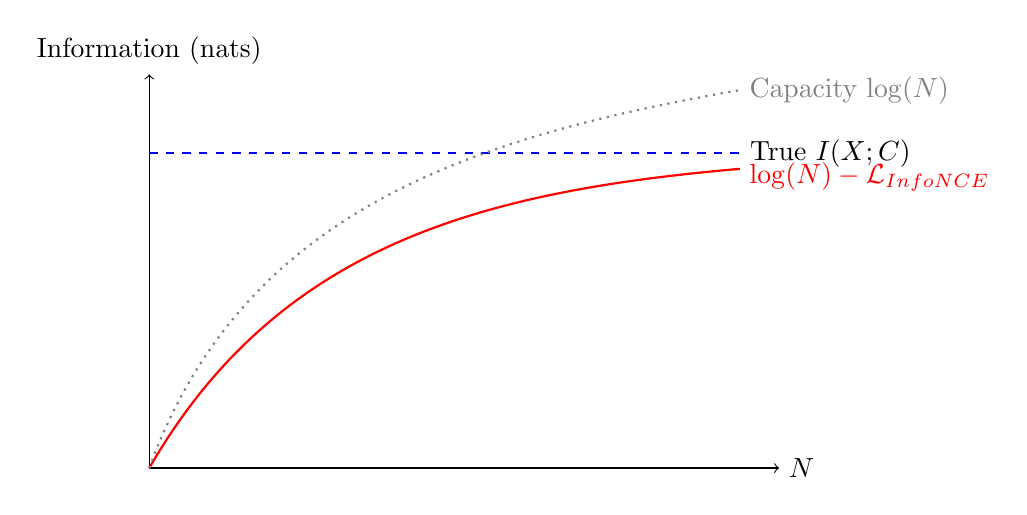
\begin{tikzpicture}
    % Axes
    \draw[->] (0,0) -- (8,0) node[right] {$N$};
    \draw[->] (0,0) -- (0,5) node[above] {Information (nats)};
    
    % True MI line
    \draw[thick, blue, dashed] (0,4) -- (7.5,4) node[right, text=black] {True $I(X; C)$};
    
    % InfoNCE bound curve
    \draw[thick, red] (0,0) to[out=60, in=185] (7.5, 3.8);
    \node[red, right] at (7.5, 3.7) {$\log(N) - \mathcal{L}_{\text{InfoNCE}}$};
    
    % Asymptote / Log N curve representation
    \draw[gray, dotted, thick] (0,0) to[out=70, in=190] (7.5, 4.8);
    \node[gray, right] at (7.5, 4.8) {Capacity $\log(N)$};
    
\end{tikzpicture}
\caption{The InfoNCE bound on Mutual Information. As the number of negative samples $N$ increases, the lower bound $\log(N) - \mathcal{L}_{\text{InfoNCE}}$ becomes tighter, asymptoting towards the true mutual information $I(X; C)$. However, the estimator is fundamentally limited by $\log(N)$, meaning extremely high MI cannot be accurately estimated with small batches.}
\label{fig:infonce_bound}
\end{figure}

\section{Numerical Example: Correlated Gaussian Variables}

To make the tightness and capacity of the bound concrete, let us calculate the theoretical InfoNCE loss for a simple numerical example. Suppose our context $c$ and future observation $x$ are jointly Gaussian with zero mean, unit variance, and correlation $\rho \in (-1, 1)$:
\begin{equation}
    \begin{pmatrix} x \\ c \end{pmatrix} \sim \mathcal{N} \left( \begin{pmatrix} 0 \\ 0 \end{pmatrix}, \begin{pmatrix} 1 & \rho \\ \rho & 1 \end{pmatrix} \right)
\end{equation}
The true mutual information between $x$ and $c$ is known analytically from differential entropy:
\begin{equation}
    I(X; C) = h(X) - h(X|C) = -\frac{1}{2} \log(1 - \rho^2)
\end{equation}
For a moderate correlation of $\rho = 0.8$, the mutual information is:
\begin{equation}
    I(X; C) = -\frac{1}{2} \log(1 - 0.64) = -\frac{1}{2} \log(0.36) \approx 0.51 \text{ nats}
\end{equation}
Now, assume we apply the InfoNCE loss using the optimal critic $f^*(x, c) = \frac{p(x|c)}{p(x)}$. By sampling $N$ points (1 positive, $N-1$ negative), we compute the empirical InfoNCE bound. Due to the $\log(N)$ capacity ceiling, if $N=2$, the maximum mutual information the bound can estimate is $\log(2) \approx 0.69$ nats. Because $0.51 < 0.69$, a batch size of $N=2$ is theoretically sufficient to estimate this mutual information without completely saturating the bound, although variance will be high. 

However, if $\rho = 0.99$, the mutual information skyrockets:
\begin{equation}
    I(X; C) = -\frac{1}{2} \log(1 - 0.99^2) \approx 1.96 \text{ nats}
\end{equation}
In this high-correlation regime, using $N=2$ negative samples will severely underestimate the mutual information, as $\log(2) - \mathcal{L}_{\text{InfoNCE}} \le 0.69 \ll 1.96$. A minimum of $N = \lceil e^{1.96} \rceil = 8$ samples is required merely to possess the theoretical capacity to upper-bound the MI, and in practice, significantly larger batch sizes (e.g., $N=256$ or $N=4096$) are necessary to reduce the variance of the estimator and tighten the bound closely to the true value.

\begin{horizon}
While Theorem \ref{thm:infonce_bound} elegantly links contrastive learning to mutual information, it is conjectured that the strict maximization of mutual information is not the sole, or even primary, driver of downstream performance in self-supervised learning. The representation capacity bound of $\log(N)$ implies that larger batch sizes strictly improve the MI bound, yet empirical studies often observe diminishing returns in downstream classification accuracy well before the MI estimator saturates. 

An open question in the field is whether there exists a more refined information-theoretic metric that accounts for the \textit{geometry} of the data manifold and the \textit{inductive bias} of the encoder $f_\theta$. Future work might show that InfoNCE implicitly optimizes an Information Bottleneck objective (Chapter 8), where the specific choice of negative sample augmentations acts as a form of targeted regularization. This would imply that the success of CPC arises precisely from discarding task-irrelevant entropy rather than uniformly maximizing $I(X; C)$.
\end{horizon}

\section{Summary}

In this chapter, we formalized Contrastive Predictive Coding (CPC) as a potent framework for unsupervised representation learning. By predicting future latent states rather than high-dimensional raw observations, CPC extracts semantic structure while filtering out local noise. We defined the Information Noise-Contrastive Estimation (InfoNCE) loss and provided a rigorous mathematical proof that minimizing this loss maximizes a lower bound on the mutual information between the context and future observations. This lower bound is fundamentally parameterized by the number of negative samples $N$. We also explored a numerical example highlighting the $\log(N)$ capacity limit of the estimator, emphasizing the necessity of large batch sizes in highly correlated environments.

\section{Exercises}

\begin{enumerate}
    \item \textbf{Optimal Critic Derivation:} In Lemma \ref{lem:optimal_critic}, we claimed that substituting the true positive sample assignment probabilities directly minimizes the InfoNCE loss. Rigorously derive this result using the calculus of variations, taking the functional derivative of the continuous integral form of $\mathcal{L}_{\text{InfoNCE}}$ with respect to the continuous function $f(\cdot, \cdot)$.
    \item \textbf{High-Dimensional Contrastive Bounds:} Suppose $x, c \in \mathbb{R}^d$ are multivariate isotropic Gaussians with covariance $\Sigma = \sigma^2 I$. Let the correlation between corresponding dimensions be $\rho$, such that $I(X; C) = -\frac{d}{2} \log(1 - \rho^2)$. As $d \to \infty$, the true mutual information grows linearly. Show analytically how the required number of negative samples $N$ must scale with $d$ to avoid the $\log(N)$ saturation phenomenon.
    \item \textbf{InfoNCE vs. MINE:} Compare the InfoNCE bound with the Mutual Information Neural Estimation (MINE) bound (Chapter 16). Which bound provides a tighter estimate for mutual information in high dimensions? Discuss the variance trade-offs between the two estimators, paying particular attention to the effects of the partition function in InfoNCE.
\end{enumerate}

% TODO-CITE: Ensure all named results are cited.
